\documentclass{article}

% content/resources/templates/preamble.tex
\usepackage[margin=0.6in]{geometry}
\author{Milav Dabgar}
\usepackage{amsmath,amssymb,amsthm}
\usepackage{booktabs}
\usepackage{multirow}
\usepackage{xcolor}
\usepackage{tcolorbox}
\tcbuselibrary{breakable,skins}
\usepackage[colorlinks=true,linkcolor=blue]{hyperref}
\usepackage{titlesec}
\usepackage{enumitem}
\usepackage{tikz}
\usepackage{pgfplots}
\usepackage{circuitikz}
\usepackage[version=4]{mhchem}
\usepackage{longtable}
\usepackage{array}
\usepackage{float}
\usepackage{caption}
\usepackage{listings}

\lstset{
  basicstyle=\small\ttfamily,
  breaklines=true,
  breakatwhitespace=false,
  postbreak=\mbox{\textcolor{red}{$\hookrightarrow$}\space},
  float=false,
  numbers=left,
  numberstyle=\tiny\color{gray},
  numbersep=10pt,
  xleftmargin=2em,
  keywordstyle=\color{blue},
  commentstyle=\color{green!60!black},
  stringstyle=\color{purple},
  backgroundcolor=\color{gray!5},
  showstringspaces=false,
  tabsize=2,
  captionpos=b,
  keepspaces=true,
  columns=flexible
}

\pgfplotsset{compat=1.18}
\usetikzlibrary{shapes,arrows,positioning,calc,patterns,decorations.pathmorphing,decorations.markings,arrows.meta}

% Color scheme
\definecolor{headcolor}{RGB}{0,102,204}
\definecolor{keycolor}{RGB}{220,20,60}
\definecolor{solutioncolor}{RGB}{34,139,34}
\definecolor{mnemoniccolor}{RGB}{148,0,211}
\definecolor{codecolor}{RGB}{0,0,100}

% Spacing
\setlength{\parskip}{3pt}
\setlist[itemize]{nosep}
\setlist[enumerate]{nosep}

% Title formatting
\titleformat{\section}{\Large\bfseries\color{headcolor}}{\thesection}{1em}{}
\titleformat{\subsection}{\large\bfseries\color{headcolor}}{\thesubsection}{1em}{}

% Pandoc tightlist compatibility
\providecommand{\tightlist}{%
  \setlength{\itemsep}{0pt}\setlength{\parskip}{0pt}}

% Pandoc longtable compatibility
\newcounter{none}
\def\thenone{}


% content/resources/templates/english-boxes.tex

% Custom environments
\newtcolorbox{solutionbox}{
 breakable,
 enhanced,
 colback=solutioncolor!5!white,
 colframe=solutioncolor!75!black,
 fonttitle=\bfseries,
 title=Solution
}

\newtcolorbox{solutionboxnobreak}{
 colback=solutioncolor!5!white,
 colframe=solutioncolor!75!black,
 fonttitle=\bfseries,
 title=Solution
}

\newtcolorbox{keyformula}{
 breakable,
 enhanced,
 colback=keycolor!5!white,
 colframe=keycolor!75!black,
 fonttitle=\bfseries,
 title=Key Formula
}

\newtcolorbox{mnemonicboxenv}{
 breakable,
 enhanced,
 colback=mnemoniccolor!5!white,
 colframe=mnemoniccolor!75!black,
 fonttitle=\bfseries,
 title=Mnemonic
}

\newcommand{\mnemonicbox}[1]{%
  \begin{mnemonicboxenv}
    #1
  \end{mnemonicboxenv}
}


% Custom commands for GTU solutions
% This file defines semantic commands for consistent formatting

% Question command with automatic formatting
\newcommand{\question}[2]{%
  \section*{Question #1}%
  \textbf{#2}%
}

% OR question variant
\newcommand{\questionor}[2]{%
  \section*{Question #1 OR}%
  \textbf{#2}%
}

% Proper table environment with caption
\newenvironment{answertable}[1]{%
  \begin{table}[htbp]
  \centering
  \caption{#1}
}{%
  \end{table}
}

% Proper figure environment for diagrams
\newenvironment{answerdiagram}[1]{%
  \begin{figure}[htbp]
  \centering
  \caption{#1}
}{%
  \end{figure}
}

% Semantic markup for key terms
\newcommand{\keyword}[1]{\textbf{#1}}
\newcommand{\code}[1]{\texttt{#1}}
\newcommand{\classname}[1]{\texttt{#1}}
\newcommand{\methodname}[1]{\texttt{#1}}

% Proper quotation marks
\newcommand{\mnemonic}[1]{``#1''}


\title{Antenna \& Wave Propagation (4341106) - Winter 2024 Solution}
\date{January 24, 2024}

\begin{document}
\maketitle

\questionmarks{1(a)}{3}{Define: (1) Directivity, (2) Gain, and (3) HPBW}

\begin{solutionbox}
\begin{tabulary}{\linewidth}{L L}
    \hline
    \textbf{Parameter} & \textbf{Definition} \\
    \hline
    \textbf{Directivity} & The ratio of radiation intensity in a given direction to the average radiation intensity in all directions. \\
    \textbf{Gain} & The ratio of power radiated in a specific direction to the power that would be radiated by an isotropic antenna with the same input power. \\
    \textbf{HPBW (Half Power Beam Width)} & The angular width of the main lobe where the power falls to half (-3dB) of its maximum value. \\
    \hline
\end{tabulary}

\begin{mnemonicbox}
    \textbf{Mnemonic:} "DGH: Direction Gets Higher power with narrow beam"
\end{mnemonicbox}
\end{solutionbox}

\questionmarks{1(b)}{4}{List the properties of electromagnetic waves}

\begin{solutionbox}
\begin{tabulary}{\linewidth}{L L}
    \hline
    \textbf{Property} & \textbf{Description} \\
    \hline
    \textbf{Transverse nature} & Electric and magnetic fields are perpendicular to each other and to direction of propagation. \\
    \textbf{Velocity} & Travel at speed of light ($3\times10^8$ m/s) in free space. \\
    \textbf{Frequency range} & Vary from few Hz to several THz. \\
    \textbf{Energy transport} & Carry energy from one point to another without need of medium. \\
    \textbf{Reflection} & Can be reflected from conducting surfaces. \\
    \textbf{Refraction} & Change direction when passing between different media. \\
    \textbf{Diffraction} & Can bend around obstacles. \\
    \textbf{Polarization} & The orientation of electric field vector. \\
    \hline
\end{tabulary}

\begin{mnemonicbox}
    \textbf{Mnemonic:} "TVFERRDP: Travel Very Fast, Energy Reflects Refracts Diffracts Polarizes"
\end{mnemonicbox}
\end{solutionbox}

\questionmarks{1(c)}{7}{Explain physical concept of generation of Electromagnetic wave}

\begin{solutionbox}
\begin{figure}[H]
    \centering
    \begin{tikzpicture}[gtu flow]
        \node[gtu block] (a) {Oscillating Electric Charge};
        \node[gtu block, right=of a] (b) {Time-varying E-Field};
        \node[gtu block, right=of b] (c) {Time-varying H-Field};
        \node[gtu block, below=of c] (d) {Time-varying E-Field};
        \node[gtu block, left=of d] (e) {Self-sustaining EM Wave};

        \draw[gtu arrow] (a) -- (b);
        \draw[gtu arrow] (b) -- (c);
        \draw[gtu arrow] (c) -- (d);
        \draw[gtu arrow] (d) -- (e);
    \end{tikzpicture}
    \caption{Generation of Electromagnetic Wave}
\end{figure}

\textbf{Process of EM Wave Generation:}
\begin{itemize}
    \item \textbf{Accelerating charge}: When electric charge accelerates, it produces time-varying electric field.
    \item \textbf{Changing electric field}: This creates a time-varying magnetic field.
    \item \textbf{Changing magnetic field}: In turn creates a time-varying electric field.
    \item \textbf{Self-propagation}: This mutual creation of fields results in self-propagating wave.
    \item \textbf{Energy transfer}: EM waves transfer energy from transmitter to receiver.
\end{itemize}

\textbf{Maxwell's Equations}: These four equations mathematically describe the generation and propagation of EM waves:
\begin{enumerate}
    \item Electric field from charges (Gauss's law).
    \item No magnetic monopoles exist.
    \item Electric fields from changing magnetic fields (Faraday's law).
    \item Magnetic fields from currents and changing electric fields (Ampere's law).
\end{enumerate}

\begin{mnemonicbox}
    \textbf{Mnemonic:} "CASES: Charges Accelerate, Self-sustaining Electric-Magnetic fields"
\end{mnemonicbox}
\end{solutionbox}

\questionmarks{1(c) OR}{7}{Explain how electromagnetic field radiated from a center fed dipole}

\begin{solutionbox}
\begin{figure}[H]
    \centering
    \begin{tikzpicture}[gtu flow]
        \node[gtu block] (gen) {RF Generator};
        \node[gtu block, right=of gen] (ant) {Center-Fed Dipole};
        \node[gtu decision, right=of ant] (curr) {Current Flow};
        \node[gtu block, above right=of curr] (elec) {Electric Field};
        \node[gtu block, below right=of curr] (mag) {Magnetic Field};
        \node[gtu state, right=of curr, xshift=3cm] (rad) {Radiation Pattern};
        
        \draw[gtu arrow] (gen) -- (ant);
        \draw[gtu arrow] (ant) -- (curr);
        \draw[gtu arrow] (curr) |- (elec);
        \draw[gtu arrow] (curr) |- (mag);
        \draw[gtu arrow] (elec) -| (rad);
        \draw[gtu arrow] (mag) -| (rad);
    \end{tikzpicture}
    \caption{Radiation from Center-Fed Dipole}
\end{figure}

\textbf{Radiation Process:}
\begin{tabulary}{\linewidth}{L L}
    \hline
    \textbf{Stage} & \textbf{Process} \\
    \hline
    \textbf{1. Current excitation} & RF signal applied at center of dipole creates alternating current. \\
    \textbf{2. Current distribution} & Sinusoidal current distribution forms along dipole, maximum at center, zero at ends. \\
    \textbf{3. Electric field} & Oscillating charges create time-varying electric field perpendicular to dipole. \\
    \textbf{4. Magnetic field} & Current flow creates magnetic field perpendicular to both dipole and electric field. \\
    \textbf{5. Near field} & Complex field pattern forms close to antenna ($< \lambda/2\pi$). \\
    \textbf{6. Far field} & At distances $> 2\lambda$, radiation stabilizes to form distinctive pattern with main and side lobes. \\
    \hline
\end{tabulary}

\textbf{Characteristics:}
\begin{itemize}
    \item \textbf{Maximum radiation}: Perpendicular to dipole axis.
    \item \textbf{Null radiation}: Along dipole axis.
    \item \textbf{Omnidirectional}: In azimuth plane (perpendicular to dipole).
    \item \textbf{Polarization}: Same as orientation of dipole.
\end{itemize}

\begin{mnemonicbox}
    \textbf{Mnemonic:} "COME-FR: Current Oscillates, Making Electric-magnetic Fields that Radiate"
\end{mnemonicbox}
\end{solutionbox}

\questionmarks{2(a)}{3}{Differentiate the resonant and non-resonant antennas}

\begin{solutionbox}
\begin{tabulary}{\linewidth}{L L L}
    \hline
    \textbf{Parameter} & \textbf{Resonant Antennas} & \textbf{Non-Resonant Antennas} \\
    \hline
    \textbf{Physical length} & Multiple of $\lambda/2$ (usually $\lambda/2$ or $\lambda$) & Not related to wavelength (typically $> \lambda$). \\
    \textbf{Standing waves} & Strong standing waves present. & Minimal standing waves. \\
    \textbf{Current distribution} & Sinusoidal with maximum at center. & Traveling wave with uniform amplitude. \\
    \textbf{Input impedance} & Resistive (at resonant frequency). & Complex (resistive + reactive). \\
    \textbf{Bandwidth} & Narrow bandwidth. & Wide bandwidth. \\
    \textbf{Examples} & Half-wave dipole, folded dipole. & Rhombic antenna, traveling wave antenna. \\
    \hline
\end{tabulary}

\begin{mnemonicbox}
    \textbf{Mnemonic:} "SIN-CIB: Size, Impedance, Narrow vs Complex, Impedance, Broad"
\end{mnemonicbox}
\end{solutionbox}

\questionmarks{2(b)}{4}{Explain Yagi antenna and discuss its radiation characteristics}

\begin{solutionbox}
\begin{figure}[H]
    \centering
    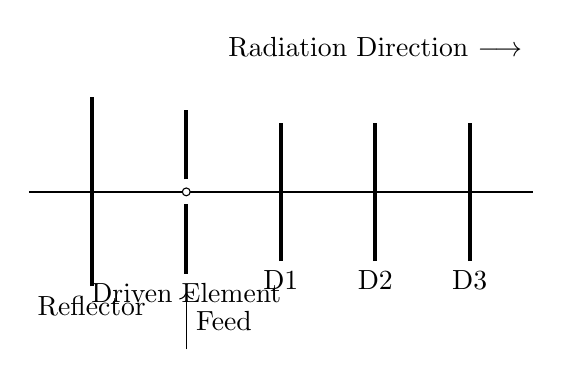
\begin{tikzpicture}[scale=0.8]
        % Boom
        \draw[thick] (0,0) -- (8,0);
        
        % Elements (vertical lines)
        % Reflector
        \draw[ultra thick] (1,-1.5) -- (1,1.5);
        \node[below] at (1,-1.5) {Reflector};
        
        % Driven Element
        \draw[ultra thick] (2.5,-1.3) -- (2.5,-0.2);
        \draw[ultra thick] (2.5,0.2) -- (2.5,1.3);
        \node[draw, circle, inner sep=1pt, fill=white] at (2.5,0) {}; % Feed point
        \node[below] at (2.5,-1.3) {Driven Element};
        \draw[->] (2.5,-2.5) -- (2.5, -1.6) node[midway, right] {Feed};
        
        % Directors
        \draw[ultra thick] (4,-1.1) -- (4,1.1);
        \node[below] at (4,-1.1) {D1};
        
        \draw[ultra thick] (5.5,-1.1) -- (5.5,1.1);
        \node[below] at (5.5,-1.1) {D2};
        
        \draw[ultra thick] (7,-1.1) -- (7,1.1);
        \node[below] at (7,-1.1) {D3};
        
        \node[above] at (5.5, 2) {Radiation Direction $\longrightarrow$};
    \end{tikzpicture}
    \caption{Yagi-Uda Antenna Structure}
\end{figure}

\textbf{Yagi Antenna Components:}
\begin{itemize}
    \item \textbf{Driven element}: Half-wave dipole connected to transmission line.
    \item \textbf{Reflector}: Slightly longer than driven element, placed behind it.
    \item \textbf{Directors}: Multiple elements shorter than driven element, placed in front.
\end{itemize}

\textbf{Radiation Characteristics:}
\begin{itemize}
    \item \textbf{Directivity}: High (7-12 dBi) with more directors.
    \item \textbf{Radiation pattern}: Unidirectional, narrow beam along director axis.
    \item \textbf{Front-to-back ratio}: 15-20 dB (good rejection of signals from rear).
    \item \textbf{Bandwidth}: Moderate (around 5\% of center frequency).
    \item \textbf{Gain}: Increases with number of directors (typically 3-20 dBi).
\end{itemize}

\begin{mnemonicbox}
    \textbf{Mnemonic:} "DRDU: Directors Radiate, Driven powers, Unidirectional beam"
\end{mnemonicbox}
\end{solutionbox}

\questionmarks{2(c)}{7}{Describe radiation characteristics of resonant wire antennas and draw the current distribution of $\lambda/2, 3\lambda/2$ and $5\lambda/2$ antenna}

\begin{solutionbox}
\begin{figure}[H]
    \centering
    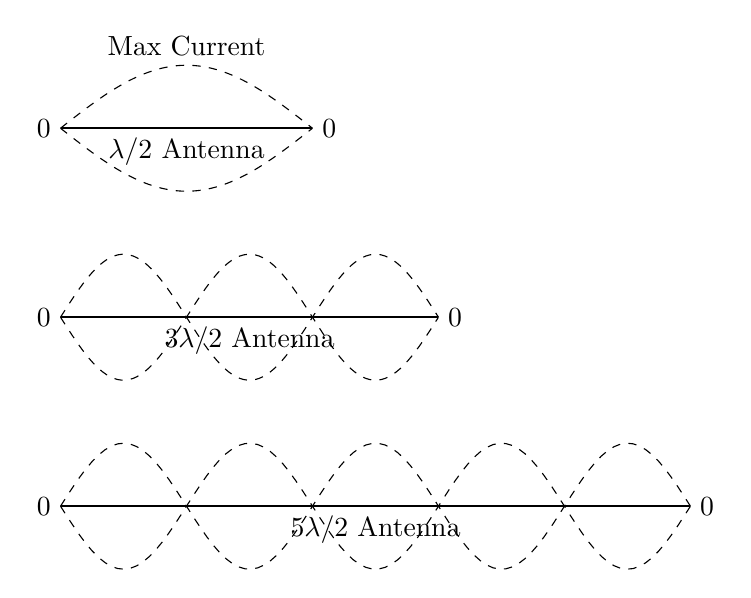
\begin{tikzpicture}[scale=0.8]
        % Lambda/2
        \begin{scope}[yshift=6cm]
            \draw[thick] (0,0) -- (4,0);
            \draw[dashed] (0,0) sin (2,1) cos (4,0);
            \draw[dashed] (0,0) sin (2,-1) cos (4,0);
            \node[below] at (2,0) {$\lambda/2$ Antenna};
            \node at (2,1.3) {Max Current};
            \node[left] at (0,0) {0};
            \node[right] at (4,0) {0};
        \end{scope}
        
        % 3Lambda/2
        \begin{scope}[yshift=3cm]
            \draw[thick] (0,0) -- (6,0);
            \draw[dashed] plot[domain=0:6, samples=100] (\x, {sin(\x*180/2)});
            \draw[dashed] plot[domain=0:6, samples=100] (\x, {-sin(\x*180/2)});
            \node[below] at (3,0) {$3\lambda/2$ Antenna};
            \node[left] at (0,0) {0};
            \node[right] at (6,0) {0};
        \end{scope}
        
        % 5Lambda/2
        \begin{scope}[yshift=0cm]
            \draw[thick] (0,0) -- (10,0);
             \draw[dashed] plot[domain=0:10, samples=100] (\x, {sin(\x*180/2)});
             \draw[dashed] plot[domain=0:10, samples=100] (\x, {-sin(\x*180/2)});
            \node[below] at (5,0) {$5\lambda/2$ Antenna};
            \node[left] at (0,0) {0};
            \node[right] at (10,0) {0};
        \end{scope}
    \end{tikzpicture}
    \caption{Current Distribution on Resonant Wire Antennas}
\end{figure}

\textbf{Radiation Characteristics of Resonant Wire Antennas:}
\begin{tabulary}{\linewidth}{L L}
    \hline
    \textbf{Characteristic} & \textbf{Description} \\
    \hline
    \textbf{Current distribution} & Sinusoidal, with maximum at center for $\lambda/2$, additional maxima for longer antennas. \\
    \textbf{Input impedance} & Approximately 73$\Omega$ for $\lambda/2$, varies for longer antennas. \\
    \textbf{Radiation pattern} & Figure-8 pattern ($\lambda/2$), more complex lobes for longer antennas. \\
    \textbf{Directivity} & 2.15 dBi for $\lambda/2$, increases with length but with multiple lobes. \\
    \textbf{Polarization} & Linear, parallel to wire orientation. \\
    \textbf{Efficiency} & High for properly constructed antennas. \\
    \hline
\end{tabulary}

\textbf{Key Points:}
\begin{itemize}
    \item $\lambda/2$ antenna has single current maximum at center.
    \item $3\lambda/2$ antenna has three half-cycles of current distribution.
    \item $5\lambda/2$ antenna has five half-cycles of current distribution.
    \item More half-wavelengths create more radiation lobes.
    \item Feed point is typically at current maximum for best impedance match.
\end{itemize}

\begin{mnemonicbox}
    \textbf{Mnemonic:} "SIMPLE: Sinusoidal In Middle Produces Lobes Efficiently"
\end{mnemonicbox}
\end{solutionbox}

\questionmarks{2(a) OR}{3}{Differentiate the broad side and end fire array antennas}

\begin{solutionbox}
\begin{tabulary}{\linewidth}{L L L}
    \hline
    \textbf{Parameter} & \textbf{Broadside Array} & \textbf{End Fire Array} \\
    \hline
    \textbf{Direction of max radiation} & Perpendicular to the array axis. & Along the array axis. \\
    \textbf{Phase difference} & 0$^\circ$ (in-phase). & 180$^\circ$ or progressive phase. \\
    \textbf{Element spacing} & Typically $\lambda/2$. & Typically $\lambda/4$ to $\lambda/2$. \\
    \textbf{Radiation pattern} & Narrow in plane containing array axis. & Narrow in plane perpendicular to array elements. \\
    \textbf{Directivity} & High, increases with number of elements. & High, increases with number of elements. \\
    \textbf{Applications} & Fixed point-to-point links. & Direction finding, radar. \\
    \hline
\end{tabulary}

\begin{mnemonicbox}
    \textbf{Mnemonic:} "BEPODS: Broadside-End, Perpendicular-Or-Direction, Spacing"
\end{mnemonicbox}
\end{solutionbox}

\questionmarks{2(b) OR}{4}{Explain loop antenna and discuss its radiation characteristics}

\begin{solutionbox}
\begin{figure}[H]
    \centering
    \begin{tikzpicture}[gtu flow]
        \node[gtu block] (root) {Loop Antenna};
        \node[gtu block, below left=of root, xshift=-1cm] (small) {Small Loop\\Circumference $< \lambda/10$};
        \node[gtu block, below right=of root, xshift=1cm] (large) {Large Loop\\Circumference $\approx \lambda$};
        
        \draw[gtu arrow] (root) -- (small);
        \draw[gtu arrow] (root) -- (large);
    \end{tikzpicture}
    \caption{Types of Loop Antennas}
\end{figure}

\textbf{Loop Antenna Characteristics:}
\begin{tabulary}{\linewidth}{L L L}
    \hline
    \textbf{Parameter} & \textbf{Small Loop} & \textbf{Large Loop} \\
    \hline
    \textbf{Current distribution} & Uniform around loop. & Varies around circumference. \\
    \textbf{Radiation pattern} & Figure-8 (perpendicular to loop plane). & More complex with multiple lobes. \\
    \textbf{Directivity} & Low (1.5 dBi). & Higher (3-4 dBi). \\
    \textbf{Polarization} & Magnetic field perpendicular to loop. & Electric field in plane of loop. \\
    \textbf{Input impedance} & Very low ($< 10\Omega$). & Higher (50-200$\Omega$). \\
    \textbf{Applications} & Direction finding, AM receivers. & HF communications, RFID. \\
    \hline
\end{tabulary}

\begin{mnemonicbox}
    \textbf{Mnemonic:} "SCALED: Size Changes Antenna's Lobes, Efficiency, and Direction"
\end{mnemonicbox}
\end{solutionbox}

\questionmarks{2(c) OR}{7}{Describe radiation characteristics of non resonant wire antennas and draw the radiation pattern of $\lambda/2, 3\lambda/2$ and $5\lambda/2$ antenna}

\begin{solutionbox}
\begin{figure}[H]
    \centering
    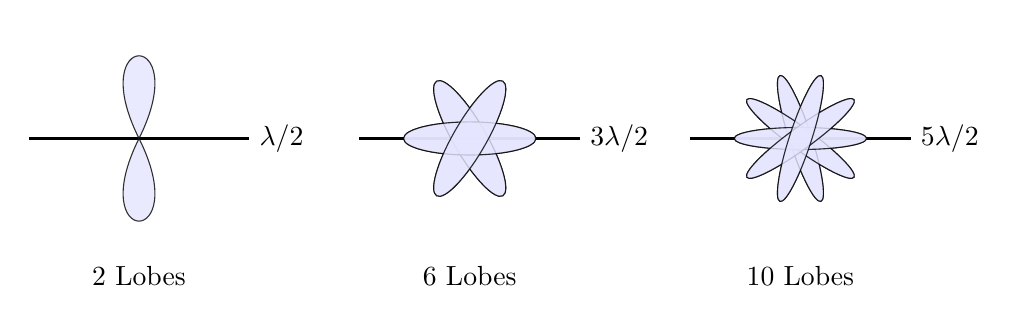
\begin{tikzpicture}[scale=0.7]
        % λ/2
        \begin{scope}
            \draw[thick] (-2,0) -- (2,0) node[right] {$\lambda/2$};
            % Figure 8 pattern
            \draw[fill=blue!10, opacity=0.8] (0,0) .. controls (1,2) and (-1,2) .. (0,0);
             \draw[fill=blue!10, opacity=0.8] (0,0) .. controls (1,-2) and (-1,-2) .. (0,0);
             \node at (0,-2.5) {2 Lobes};
        \end{scope}

        % 3λ/2
        \begin{scope}[xshift=6cm]
            \draw[thick] (-2,0) -- (2,0) node[right] {$3\lambda/2$};
            % 3 lobes each side (simplified representation)
            \foreach \a in {30, 90, 150, 210, 270, 330}
                \draw[fill=blue!10, opacity=0.8, rotate=\a] (0,0) ellipse (0.3 and 1.2);
            \node at (0,-2.5) {6 Lobes};
        \end{scope}

        % 5λ/2
        \begin{scope}[xshift=12cm]
            \draw[thick] (-2,0) -- (2,0) node[right] {$5\lambda/2$};
             % 5 lobes each side
            \foreach \a in {18, 54, 90, 126, 162, 198, 234, 270, 306, 342}
                \draw[fill=blue!10, opacity=0.8, rotate=\a] (0,0) ellipse (0.2 and 1.2);
            \node at (0,-2.5) {10 Lobes};
        \end{scope}
    \end{tikzpicture}
    \caption{Radiation Patterns of Resonant Wire Antennas (Simplified)}
\end{figure}

\textbf{Non-Resonant Wire Antenna Characteristics:}
\begin{tabulary}{\linewidth}{L L}
    \hline
    \textbf{Characteristic} & \textbf{Description} \\
    \hline
    \textbf{Current distribution} & Traveling waves with minimal standing waves. \\
    \textbf{Termination} & Usually terminated with resistive load to prevent reflections. \\
    \textbf{Bandwidth} & Wide bandwidth operation. \\
    \textbf{Input impedance} & More constant across frequency range. \\
    \textbf{Radiation pattern} & $\lambda/2$: Single main lobe on each side (tilted). \\
    & $3\lambda/2$: Three main lobes on each side (tilted). \\
    & $5\lambda/2$: Five main lobes on each side (tilted). \\
    \textbf{Directivity} & Increases with length but divided among multiple lobes. \\
    \textbf{Efficiency} & Lower than resonant antennas due to resistive termination. \\
    \hline
\end{tabulary}

\begin{mnemonicbox}
    \textbf{Mnemonic:} "TRIBE-WL: Traveling Resistance Improves Bandwidth, Efficiency Worse, Lobes multiply"
\end{mnemonicbox}
\end{solutionbox}

\questionmarks{3(a)}{3}{Write short note on micro strip (patch) antenna}

\begin{solutionbox}
\begin{figure}[H]
    \centering
    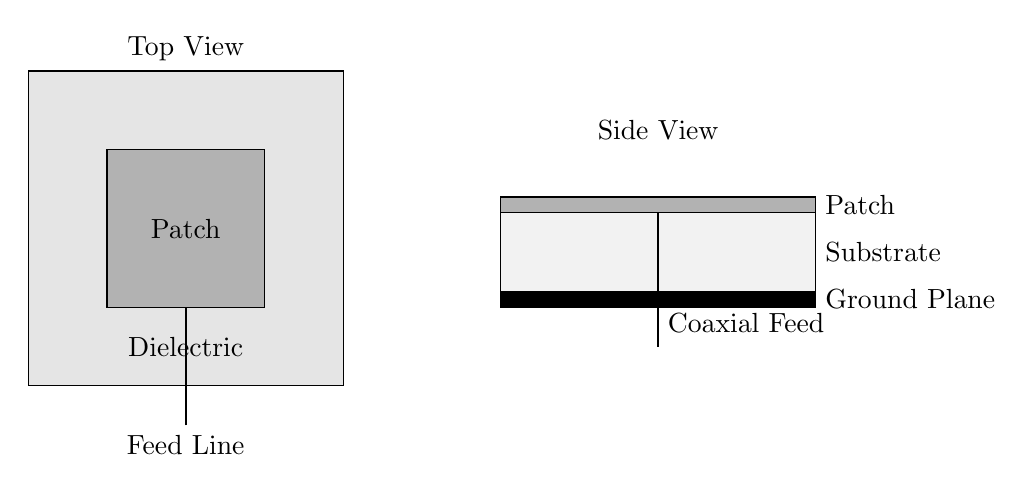
\begin{tikzpicture}
        % Top View
        \begin{scope}
            \draw[fill=gray!20] (0,0) rectangle (4,4);
            \draw[fill=gray!60] (1,1) rectangle (3,3);
            \node at (2,2) {Patch};
            \node at (2,0.5) {Dielectric};
            \draw[thick] (2, -0.5) -- (2, 1);
            \node[below] at (2,-0.5) {Feed Line};
            \node[above] at (2,4) {Top View};
        \end{scope}
        
        % Side View
        \begin{scope}[xshift=6cm, yshift=1cm]
            \draw[fill=gray!60] (0,1.2) rectangle (4,1.4); \node[right] at (4,1.3) {Patch};
            \draw[fill=gray!10] (0,0.2) rectangle (4,1.2); \node[right] at (4,0.7) {Substrate};
            \draw[fill=black] (0,0) rectangle (4,0.2); \node[right] at (4,0.1) {Ground Plane};
            \draw[thick] (2,-0.5) -- (2, 1.2); \node[right] at (2,-0.2) {Coaxial Feed};
            \node[above] at (2,2) {Side View};
        \end{scope}
    \end{tikzpicture}
    \caption{Microstrip Patch Antenna Structure}
\end{figure}

\textbf{Microstrip Patch Antenna:}
\begin{itemize}
    \item \textbf{Structure}: Metal patch on dielectric substrate with ground plane.
    \item \textbf{Size}: Typically $\lambda/2 \times \lambda/2$ or $\lambda/2 \times \lambda/4$.
    \item \textbf{Feed methods}: Microstrip line, coaxial probe, aperture coupling.
    \item \textbf{Radiation}: From fringing fields at patch edges.
    \item \textbf{Polarization}: Linear or circular depending on patch shape.
    \item \textbf{Bandwidth}: Narrow (3-5\% of center frequency).
    \item \textbf{Applications}: Mobile devices, satellites, aircraft, RFID.
\end{itemize}

\begin{mnemonicbox}
    \textbf{Mnemonic:} "SLIM-PCB: Small, Lightweight, Integrable Microwave Printed Circuit Board"
\end{mnemonicbox}
\end{solutionbox}

\questionmarks{3(b)}{4}{Explain helical antenna and discuss its radiation characteristics}

\begin{solutionbox}
\begin{figure}[H]
    \centering
    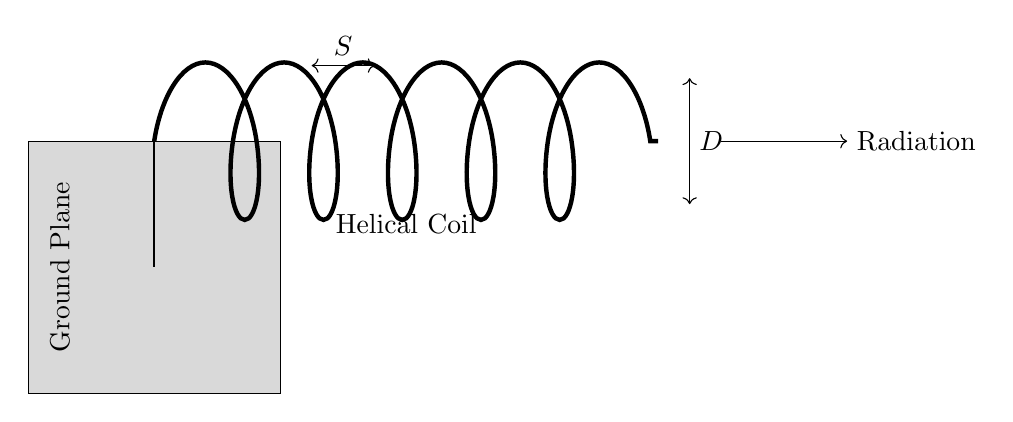
\begin{tikzpicture}[scale=0.8]
        % Ground plane
        \draw[fill=gray!30] (-2,0) rectangle (2,4);
        \node[rotate=90] at (-1.5, 2) {Ground Plane};
        
        % Helix
        \draw[ultra thick, decoration={coil, aspect=0.4, segment length=10mm, amplitude=10mm}, decorate] (0,4) -- (8,4);
        \draw[thick] (0,4) -- (0,2); % Feed connection
        \node[below] at (4,3) {Helical Coil};
        
        % Parameters
        \draw[<->] (2.5, 5.2) -- (3.5, 5.2) node[midway, above] {$S$};
        \draw[<->] (8.5, 3) -- (8.5, 5) node[midway, right] {$D$};
        \draw[->] (9, 4) -- (11, 4) node[right] {Radiation};
    \end{tikzpicture}
    \caption{Helical Antenna (Axial Mode)}
\end{figure}

\textbf{Helical Antenna Characteristics:}
\begin{tabulary}{\linewidth}{L L L}
    \hline
    \textbf{Parameter} & \textbf{Normal Mode} & \textbf{Axial Mode} \\
    \hline
    \textbf{Helix circumference} & Small ($< \lambda/\pi$). & About $\lambda$. \\
    \textbf{Radiation pattern} & Omnidirectional (like dipole). & Directional (end-fire). \\
    \textbf{Polarization} & Linear, perpendicular to helix axis. & Circular (RHCP or LHCP). \\
    \textbf{Input impedance} & High (120-200$\Omega$). & 100-200$\Omega$. \\
    \textbf{Bandwidth} & Narrow. & Wide (up to 70\%). \\
    \textbf{Applications} & Mobile phones, FM radio. & Satellite comms, space telemetry. \\
    \hline
\end{tabulary}

\begin{mnemonicbox}
    \textbf{Mnemonic:} "NASA-CP: Normal Axial Spacing Affects Circular Polarization"
\end{mnemonicbox}
\end{solutionbox}

\questionmarks{3(c)}{7}{Explain horn antenna and discuss its radiation characteristics}

\begin{solutionbox}
\begin{figure}[H]
    \centering
    \begin{tikzpicture}[gtu flow]
        \node[gtu block] (root) {Horn Antenna};
        \node[gtu block, below left=of root, xshift=-2cm] (e) {E-plane Horn};
        \node[gtu block, below left=of root] (h) {H-plane Horn};
        \node[gtu block, below right=of root] (p) {Pyramidal Horn};
        \node[gtu block, below right=of root, xshift=2cm] (c) {Conical Horn};
        
        \draw[gtu arrow] (root) -- (e);
        \draw[gtu arrow] (root) -- (h);
        \draw[gtu arrow] (root) -- (p);
        \draw[gtu arrow] (root) -- (c);
    \end{tikzpicture}
    \caption{Types of Horn Antennas}
\end{figure}

\begin{figure}[H]
    \centering
    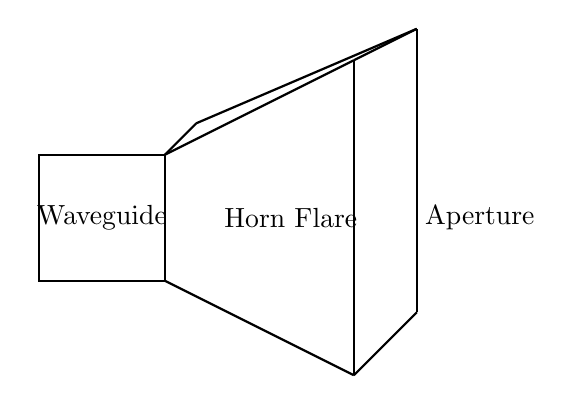
\begin{tikzpicture}[scale=0.8]
        % Waveguide section
        \draw[thick] (0,1) -- (2,1) -- (2,-1) -- (0,-1) -- cycle;
        \node at (1,0) {Waveguide};
        
        % Horn section (Pyramidal flare)
        \draw[thick] (2,1) -- (5,2.5);
        \draw[thick] (2,-1) -- (5,-2.5);
        \draw[thick] (5,2.5) -- (5,-2.5);
        
        % Perspective lines for 3D effect
        \draw[thick] (2,1) -- (2.5, 1.5);
        \draw[thick] (5,2.5) -- (6, 3);
        \draw[thick] (2.5, 1.5) -- (6, 3);
        \draw[thick] (6,3) -- (6, -1.5);
        \draw[thick] (5, -2.5) -- (6, -1.5);
        
        \node at (4, 0) {Horn Flare};
        \node at (7, 0) {Aperture};
    \end{tikzpicture}
    \caption{Pyramidal Horn Antenna Structure}
\end{figure}

\textbf{Horn Antenna Characteristics:}
\begin{tabulary}{\linewidth}{L L}
    \hline
    \textbf{Characteristic} & \textbf{Description} \\
    \hline
    \textbf{Operating principle} & Gradual transition from waveguide to free space. \\
    \textbf{Frequency range} & Microwave and mm-wave (1-300 GHz). \\
    \textbf{Directivity} & Medium to high (10-20 dBi). \\
    \textbf{Radiation pattern} & Directional with main lobe in forward direction. \\
    \textbf{Beamwidth} & E-plane: 40-50$^\circ$, H-plane: 40-50$^\circ$. \\
    \textbf{Polarization} & Linear (matches waveguide). \\
    \textbf{Bandwidth} & Very wide ($>100\%$). \\
    \textbf{Efficiency} & Very high ($>90\%$). \\
    \textbf{Applications} & Radar, satellite communications, EMC testing. \\
    \hline
\end{tabulary}

\begin{mnemonicbox}
    \textbf{Mnemonic:} "POWER-HF: Pyramidal Or Waveguide Extended, Radiates High Frequencies"
\end{mnemonicbox}
\end{solutionbox}

\questionmarks{3(a) OR}{3}{Write short note on slot antenna}

\begin{solutionbox}
\begin{figure}[H]
    \centering
    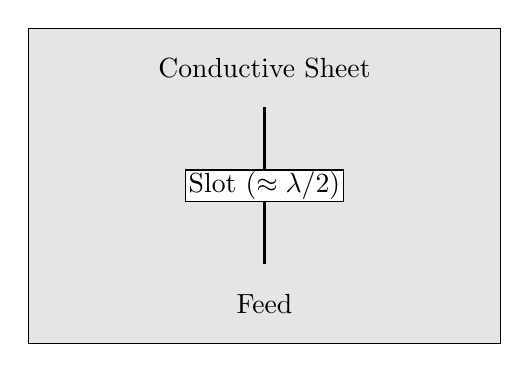
\begin{tikzpicture}
        % Conductive sheet
        \draw[fill=gray!20] (0,0) rectangle (6,4);
        % Slot
        \draw[fill=white] (2, 1.8) rectangle (4, 2.2);
        \node at (3, 2) {Slot ($\approx \lambda/2$)};
        \node at (3, 3.5) {Conductive Sheet};
        
        % Feed
        \draw[thick] (3, 1.8) -- (3, 1);
        \draw[thick] (3, 2.2) -- (3, 3);
        \node at (3, 0.5) {Feed};
    \end{tikzpicture}
    \caption{Slot Antenna}
\end{figure}

\textbf{Slot Antenna:}
\begin{itemize}
    \item \textbf{Structure}: Narrow slot cut in conductive sheet/plane.
    \item \textbf{Size}: Typically $\lambda/2$ long for resonance.
    \item \textbf{Feed method}: Across the slot at center or offset.
    \item \textbf{Radiation pattern}: Similar to dipole but rotated 90$^\circ$ (Babinet's principle).
    \item \textbf{Polarization}: Linear, perpendicular to slot length.
    \item \textbf{Impedance}: High (several hundred ohms).
    \item \textbf{Applications}: Aircraft, satellites, base stations.
\end{itemize}

\begin{mnemonicbox}
    \textbf{Mnemonic:} "SCRAP: Slot Cut Radiates Alternating Polarization"
\end{mnemonicbox}
\end{solutionbox}

\questionmarks{3(b) OR}{4}{Explain parabolic reflector antenna and discuss its radiation characteristics}

\begin{solutionbox}
\begin{figure}[H]
    \centering
    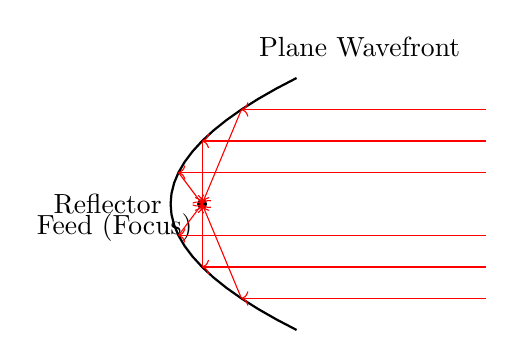
\begin{tikzpicture}[scale=0.8]
        % Parabola
        \draw[thick] plot[domain=-2:2] (\x*\x/2, \x);
        
        % Feed
        \draw[fill=black] (0.5, 0) circle (2pt) node[below left] {Feed (Focus)};
        
        % Rays
        \foreach \h in {-1.5, -1, -0.5, 0.5, 1, 1.5} {
            % Incoming
            \draw[->, red] (5, \h) -- ({\h*\h/2}, \h);
            % Reflected to focus
            \draw[->, red] ({\h*\h/2}, \h) -- (0.5, 0);
        }
        
        \node at (3, 2.5) {Plane Wavefront};
        \node at (-1, 0) {Reflector};
    \end{tikzpicture}
    \caption{Parabolic Reflector Ray Tracing}
\end{figure}

\textbf{Parabolic Reflector Antenna Characteristics:}
\begin{tabulary}{\linewidth}{L L}
    \hline
    \textbf{Characteristic} & \textbf{Description} \\
    \hline
    \textbf{Operating principle} & Focuses parallel incoming waves to focal point (receiving). \\
    \textbf{Frequency range} & From UHF to millimeter waves (300 MHz - 300 GHz). \\
    \textbf{Directivity} & Very high (30-40 dBi for large dishes). \\
    \textbf{Radiation pattern} & Highly directional, narrow main beam. \\
    \textbf{Beamwidth} & Inversely proportional to diameter ($\theta \approx 70\lambda/D$ degrees). \\
    \textbf{Feed types} & Prime focus, Cassegrain, Gregorian, offset. \\
    \textbf{Efficiency} & 50-70\% depending on feed design and blockage. \\
    \hline
\end{tabulary}

\begin{mnemonicbox}
    \textbf{Mnemonic:} "FIND-SHF: Focused, Intense Narrow Directivity for Super High Frequencies"
\end{mnemonicbox}
\end{solutionbox}

\questionmarks{3(c) OR}{7}{Describe V and inverted V antenna}

\begin{solutionbox}
\begin{figure}[H]
    \centering
    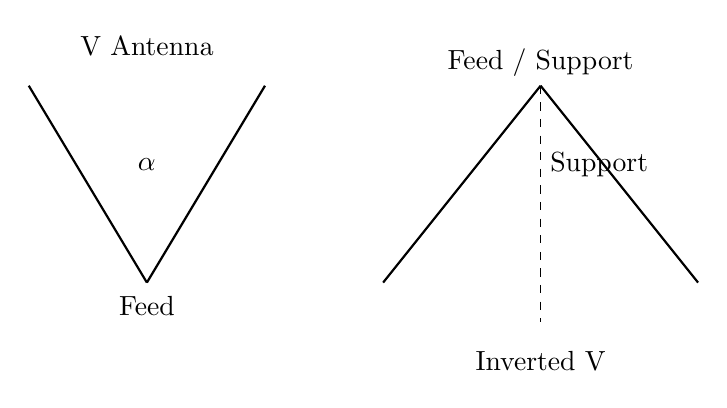
\begin{tikzpicture}
        % V Antenna
        \begin{scope}
            \draw[thick] (0,0) -- ( -1.5, 2.5);
            \draw[thick] (0,0) -- ( 1.5, 2.5);
            \node at (0, -0.3) {Feed};
            \node at (0, 3) {V Antenna};
            \node at (0, 1.5) {$\alpha$};
        \end{scope}
        
        % Inverted V
        \begin{scope}[xshift=5cm, yshift=2.5cm]
            \draw[thick] (0,0) -- (-2, -2.5);
            \draw[thick] (0,0) -- (2, -2.5);
            \draw[dashed] (0,0) -- (0, -3); % Support
            \node[right] at (0, -1) {Support};
            \node[above] at (0,0) {Feed / Support};
            \node at (0, -3.5) {Inverted V};
        \end{scope}
    \end{tikzpicture}
    \caption{V and Inverted V Antennas}
\end{figure}

\textbf{Comparison:}
\begin{tabulary}{\linewidth}{L L L}
    \hline
    \textbf{Characteristic} & \textbf{V Antenna} & \textbf{Inverted V Antenna} \\
    \hline
    \textbf{Construction} & Two equal length wires in V-shape. & Bent dipole in inverted V-shape. \\
    \textbf{Angle} & 10-90$^\circ$ (affects directivity). & 90-120$^\circ$ typically. \\
    \textbf{Leg Length} & Multiple wavelengths ($1-6\lambda$). & $\lambda/4$ each (total $\lambda/2$). \\
    \textbf{Pattern} & Bidirectional/Unidirectional. & Omnidirectional (mostly). \\
    \textbf{Impedance} & 300-900$\Omega$. & Lower ($\approx 50\Omega$). \\
    \textbf{Mounting} & Horizontal. & Vertical (single center support). \\
    \hline
\end{tabulary}

\begin{mnemonicbox}
    \textbf{Mnemonic:} "VOVO: V Outward (radiation), V One-support (inverted)"
\end{mnemonicbox}
\end{solutionbox}


\questionmarks{4(a)}{3}{Define: (1) Reflection, (2) Refraction and (3) Diffraction}

\begin{solutionbox}
\begin{tabulary}{\linewidth}{L L}
    \hline
    \textbf{Phenomenon} & \textbf{Definition} \\
    \hline
    \textbf{Reflection} & The bouncing back of electromagnetic waves when they strike a boundary between two different media without penetrating the second medium. \\
    \textbf{Refraction} & The bending of electromagnetic waves when they pass from one medium to another due to change in wave velocity. \\
    \textbf{Diffraction} & The bending of electromagnetic waves around obstacles or through openings, allowing waves to propagate into shadowed regions. \\
    \hline
\end{tabulary}

\begin{mnemonicbox}
    \textbf{Mnemonic:} "RRD: Rays Rebound, Redirect, Disperse"
\end{mnemonicbox}
\end{solutionbox}

\questionmarks{4(b)}{4}{List HAM radio application for communication}

\begin{solutionbox}
\begin{tabulary}{\linewidth}{L L}
    \hline
    \textbf{Application Category} & \textbf{Specific Applications} \\
    \hline
    \textbf{Emergency communications} & Disaster relief, emergency response, weather reporting. \\
    \textbf{Public service} & Community events, search and rescue, traffic monitoring. \\
    \textbf{Technical experimentation} & Antenna design, propagation studies, digital modes testing. \\
    \textbf{International goodwill} & DX communication, contesting, international friendship. \\
    \textbf{Personal recreation} & Casual conversations, hobby groups, radio clubs. \\
    \textbf{Educational outreach} & School programs, STEM activities, training new operators. \\
    \textbf{Space communication} & Satellite operation, ISS contact, EME (moon bounce). \\
    \textbf{Digital communication} & APRS, packet radio, FT8, RTTY, PSK31. \\
    \hline
\end{tabulary}

\begin{mnemonicbox}
    \textbf{Mnemonic:} "EPTIPS-D: Emergency, Public, Technical, International, Personal, Space, Digital"
\end{mnemonicbox}
\end{solutionbox}

\questionmarks{4(c)}{7}{Explain ionosphere's layers and sky wave propagation}

\begin{solutionbox}
\begin{figure}[H]
    \centering
    \begin{tikzpicture}[gtu flow]
        \node[gtu block] (tx) {Transmitter};
        \node[gtu state, above=of tx, yshift=1cm] (ion) {Ionosphere};
        \node[gtu block, right=of tx, xshift=4cm] (rx) {Receiver};
        
        \node[draw, dashed, fit=(ion), inner sep=1cm, label=above:Layers] (layers) {};
        
        \node[above=of layers.south, yshift=0.5cm] (d) {D Layer (60-90 km)};
        \node[above=of d] (e) {E Layer (90-120 km)};
        \node[above=of e] (f1) {F1 Layer (170-220 km)};
        \node[above=of f1] (f2) {F2 Layer (250-450 km)};
        
        \draw[->, wave] (tx) -- (f2.west) node[midway, left] {Sky Wave};
        \draw[->, wave] (f2.east) -- (rx);
    \end{tikzpicture}
    \caption{Ionospheric Layers and Sky Wave Propagation}
\end{figure}

\textbf{Ionospheric Layers:}
\begin{tabulary}{\linewidth}{L L L L}
    \hline
    \textbf{Layer} & \textbf{Altitude} & \textbf{Characteristics} & \textbf{Effect on Radio Waves} \\
    \hline
    \textbf{D Layer} & 60-90 km & Low ionization, exists only during daylight. & Absorbs LF/MF signals, minimal refraction. \\
    \textbf{E Layer} & 90-120 km & Medium ionization, stronger during day. & Refracts HF waves up to 5 MHz. \\
    \textbf{F1 Layer} & 170-220 km & Present only during day, merges with F2 at night. & Refracts higher HF frequencies. \\
    \textbf{F2 Layer} & 250-450 km & Highest ionization, present day and night. & Main layer for long-distance HF communication. \\
    \hline
\end{tabulary}

\textbf{Sky Wave Propagation Parameters:}
\begin{itemize}
    \item \textbf{Virtual Height}: Apparent height where reflection seems to occur (higher than actual due to gradual refraction).
    \item \textbf{Critical Frequency}: Maximum frequency that can be reflected when transmitted vertically.
    \item \textbf{Maximum Usable Frequency (MUF)}: Highest frequency that can be used for communication between two points.
    \item \textbf{Skip Distance}: Minimum distance from transmitter where sky waves return to Earth.
    \item \textbf{Lowest Usable Frequency (LUF)}: Minimum frequency that provides reliable communication.
    \item \textbf{Optimum Working Frequency (OWF)}: Typically 85\% of MUF, provides most reliable communication.
\end{itemize}

\begin{mnemonicbox}
    \textbf{Mnemonic:} "DEFMSL: During day, Every Frequency Makes Somewhat Longer paths"
\end{mnemonicbox}
\end{solutionbox}

\questionmarks{4(a) OR}{3}{Define: (1) MUF, (2) LUF and (3) Skip distance}

\begin{solutionbox}
\begin{tabulary}{\linewidth}{L L}
    \hline
    \textbf{Term} & \textbf{Definition} \\
    \hline
    \textbf{MUF (Maximum Usable Frequency)} & The highest frequency that can be used for reliable communication between two specific points via ionospheric reflection. \\
    \textbf{LUF (Lowest Usable Frequency)} & The minimum frequency that provides adequate signal strength for reliable communication despite D-layer absorption. \\
    \textbf{Skip Distance} & The minimum distance from a transmitter at which a sky wave of a specific frequency returns to Earth. \\
    \hline
\end{tabulary}

\begin{mnemonicbox}
    \textbf{Mnemonic:} "MLS: Maximum frequency Leaps, Lowest frequency Seeps, Skip distance Spans"
\end{mnemonicbox}
\end{solutionbox}

\questionmarks{4(b) OR}{4}{List HAM radio digital modes of communication}

\begin{solutionbox}
\begin{tabulary}{\linewidth}{L L L}
    \hline
    \textbf{Digital Mode} & \textbf{Description} & \textbf{Typical Frequency Bands} \\
    \hline
    \textbf{FT8} & Low power, narrow bandwidth, automated exchange. & HF bands (especially 20m, 40m, 80m). \\
    \textbf{PSK31} & Phase Shift Keying, keyboard-to-keyboard. & HF bands (especially 20m, 40m). \\
    \textbf{RTTY} & Radio Teletype, oldest digital mode. & HF bands. \\
    \textbf{APRS} & Automatic Packet Reporting System, position reporting. & VHF (typically 144.39 MHz in US). \\
    \textbf{SSTV} & Slow Scan Television, image transmission. & HF bands (especially 20m). \\
    \textbf{JT65/JT9} & Weak signal modes for EME and DX. & HF and VHF bands. \\
    \textbf{WINLINK} & Email over radio. & HF and VHF bands. \\
    \textbf{DMR} & Digital Mobile Radio, voice digital mode. & VHF and UHF bands. \\
    \hline
\end{tabulary}

\begin{mnemonicbox}
    \textbf{Mnemonic:} "PRAW-JDW: PSK, RTTY, APRS, WINLINK, JT65, DMR"
\end{mnemonicbox}
\end{solutionbox}

\questionmarks{4(c) OR}{7}{Explain space wave propagation}

\begin{solutionbox}
\begin{figure}[H]
    \centering
    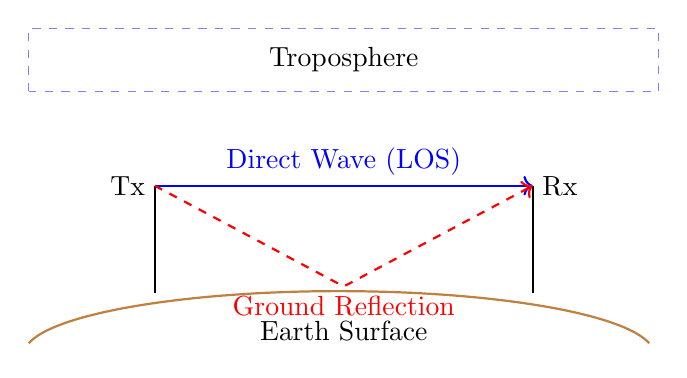
\begin{tikzpicture}[scale=0.8]
        % Earth
        \draw[thick, brown] (-5,0) arc (170:10:5 and 1); 
        \node[below] at (0,0.5) {Earth Surface};
        
        % Towers
        \draw[thick] (-3, 0.8) -- (-3, 2.5);
        \node[left] at (-3, 2.5) {Tx};
        \draw[thick] (3, 0.8) -- (3, 2.5);
        \node[right] at (3, 2.5) {Rx};
        
        % Direct Wave
        \draw[->, thick, blue] (-3, 2.5) -- (3, 2.5) node[midway, above] {Direct Wave (LOS)};
        
        % Reflected Wave
        \draw[->, thick, red, dashed] (-3, 2.5) -- (0, 0.9) -- (3, 2.5);
        \node[below, red] at (0, 0.9) {Ground Reflection};
        
        % Troposphere
        \draw[dashed, blue!50] (-5, 4) rectangle (5, 5);
        \node at (0, 4.5) {Troposphere};
    \end{tikzpicture}
    \caption{Space Wave Propagation Mechanisms}
\end{figure}

\textbf{Space Wave Propagation:}
Space wave propagation refers to radio waves that travel through the troposphere (lower atmosphere) rather than via ionospheric reflection. It includes:
\begin{enumerate}
    \item \textbf{Direct wave}: Travels in straight line from transmitter to receiver (line-of-sight).
    \item \textbf{Ground-reflected wave}: Reflects off Earth's surface before reaching receiver.
    \item \textbf{Surface wave}: Follows Earth's curvature due to diffraction.
\end{enumerate}

\textbf{Types of Space Wave Propagation:}
\begin{itemize}
    \item \textbf{Tropospheric Scatter Propagation}:
    \begin{itemize}
        \item \textbf{Mechanism}: Signal scattering by irregularities in troposphere.
        \item \textbf{Frequency range}: VHF, UHF, SHF (100 MHz - 10 GHz).
        \item \textbf{Distance}: 100-800 km (beyond horizon).
    \end{itemize}
    \item \textbf{Duct Propagation}:
    \begin{itemize}
        \item \textbf{Mechanism}: Trapping of waves in atmospheric ducts (layers with abnormal refractive index).
        \item \textbf{Distance}: Up to 2000 km (far beyond horizon).
    \end{itemize}
\end{itemize}

\textbf{Factors Affecting Space Wave Propagation:}
\begin{itemize}
    \item \textbf{Height of antennas}: Higher antennas increase range.
    \item \textbf{Frequency}: Higher frequencies experience less diffraction.
    \item \textbf{Terrain}: Obstacles block signals (Fresnel zone clearance needed).
    \item \textbf{Weather}: Temperature inversions, humidity affect ducting.
    \item \textbf{Earth's curvature}: Limits line-of-sight distance.
\end{itemize}

\begin{mnemonicbox}
    \textbf{Mnemonic:} "DRIFT-SD: Direct Routes, Irregular Formations of Troposphere, Scatter and Ducts"
\end{mnemonicbox}
\end{solutionbox}

\questionmarks{5(a)}{3}{Define: (1) Beam area (2) Beam efficiency, and (3) Effective aperture}

\begin{solutionbox}
\begin{tabulary}{\linewidth}{L L}
    \hline
    \textbf{Parameter} & \textbf{Definition} \\
    \hline
    \textbf{Beam Area} & The solid angle through which all of the power radiated by the antenna would pass if the radiation intensity was constant at its maximum value. \\
    \textbf{Beam Efficiency} & The ratio of power radiated in the main beam to the total power radiated by the antenna. \\
    \textbf{Effective Aperture} & The ratio of power received by the antenna to the power density of the incident wave. \\
    \hline
\end{tabulary}

\begin{mnemonicbox}
    \textbf{Mnemonic:} "BEA: Beam area Encloses, efficiency Excludes sidelobes, Aperture Extracts power"
\end{mnemonicbox}
\end{solutionbox}

\questionmarks{5(b)}{4}{Describe need of smart antenna}

\begin{solutionbox}
\begin{figure}[H]
    \centering
    \begin{tikzpicture}[gtu flow]
        \node[gtu block] (array) {Antenna Array};
        \node[gtu process, right=of array] (sp) {Signal Processing};
        \node[gtu decision, right=of sp] (algo) {Adaptive Algorithm};
        \node[gtu block, right=of algo] (beam) {Beamforming};
        
        \node[gtu state, below=of beam, xshift=-2cm] (int) {Interference Reduction};
        \node[gtu state, below=of beam] (cov) {Coverage Enhancement};
        \node[gtu state, below=of beam, xshift=2cm] (cap) {Capacity Increase};
        
        \draw[gtu arrow] (array) -- (sp);
        \draw[gtu arrow] (sp) -- (algo);
        \draw[gtu arrow] (algo) -- (beam);
        \draw[gtu arrow] (beam) -- (int);
        \draw[gtu arrow] (beam) -- (cov);
        \draw[gtu arrow] (beam) -- (cap);
    \end{tikzpicture}
    \caption{Smart Antenna System Concept}
\end{figure}

\textbf{Need for Smart Antennas:}
\begin{tabulary}{\linewidth}{L L}
    \hline
    \textbf{Need} & \textbf{Description} \\
    \hline
    \textbf{Spectrum efficiency} & Reuse frequencies more effectively in same geographic area. \\
    \textbf{Capacity enhancement} & Support more users in same bandwidth through spatial separation. \\
    \textbf{Coverage extension} & Increase range by focusing energy in desired directions. \\
    \textbf{Interference reduction} & Minimize effects of co-channel interference and jammers. \\
    \textbf{Energy efficiency} & Reduce transmitted power by focusing energy only where needed. \\
    \textbf{Multipath mitigation} & Reduce fading by selecting optimal signal paths. \\
    \textbf{Location services} & Enable direction finding and positioning applications. \\
    \textbf{Signal quality} & Improve SNR through spatial filtering. \\
    \hline
\end{tabulary}

\begin{mnemonicbox}
    \textbf{Mnemonic:} "SLIM-ACES: Spectrum efficiency, Location services, Interference reduction, Multipath mitigation, Adaptive beams, Capacity, Energy, Signal quality"
\end{mnemonicbox}
\end{solutionbox}

\questionmarks{5(c)}{7}{Draw the DTH Receiver indoor and outdoor black diagram and discuss its functions}

\begin{solutionbox}
\begin{figure}[H]
    \centering
    \begin{tikzpicture}[gtu flow]
        % Outdoor Unit
        \node[draw, dashed, inner sep=0.5cm, fill=gray!5, label=above:Outdoor Unit] (outdoor) {
            \begin{tikzpicture}
                \node[gtu block] (dish) {Satellite Dish};
                \node[gtu block, below=of dish] (lnb) {LNB};
                \draw[gtu arrow] (dish) -- (lnb);
            \end{tikzpicture}
        };
        
        % Indoor Unit
        \node[draw, dashed, inner sep=0.5cm, fill=gray!5, label=above:Indoor Unit, right=of outdoor, xshift=2cm] (indoor) {
            \begin{tikzpicture}
                \node[gtu process] (tuner) {Tuner/Demodulator};
                \node[gtu block, below=of tuner] (mpeg) {MPEG Decoder};
                \node[gtu decision, right=of tuner] (cam) {Conditional Access};
                \node[gtu block, below=of cam] (ctrl) {System Controller};
                
                \draw[gtu arrow] (tuner) -- (mpeg);
                \draw[gtu arrow] (tuner) -- (cam);
                \draw[gtu arrow] (ctrl) -- (tuner);
                \draw[gtu arrow] (ctrl) -- (mpeg);
            \end{tikzpicture}
        };
        
        % TV
        \node[gtu state, right=of indoor] (tv) {TV};
        
        % Connections
        \draw[gtu arrow] (outdoor.east |- lnb) -- (indoor.west |- tuner) node[midway, above] {Coaxial Cable};
        \draw[gtu arrow] (indoor.east |- mpeg) -- (tv.west);
        
    \end{tikzpicture}
    \caption{DTH Receiver System Block Diagram}
\end{figure}

\textbf{DTH Receiver System Components and Functions:}

\textbf{Outdoor Unit Components:}
\begin{itemize}
    \item \textbf{Satellite Dish}: Collects and reflects weak satellite signals to focal point.
    \item \textbf{LNB (Low Noise Block)}: Receives signals from dish, amplifies them with minimal noise addition, and converts high frequency (10-12 GHz) to lower IF frequency (950-2150 MHz).
\end{itemize}

\textbf{Indoor Unit Components:}
\begin{itemize}
    \item \textbf{Tuner/Demodulator}: Selects desired channel frequency, demodulates signal to extract digital data stream.
    \item \textbf{MPEG-2/4 Decoder}: Decodes compressed video/audio signals into viewable/audible content.
    \item \textbf{Conditional Access Module}: Provides security and decryption for subscribed channels.
    \item \textbf{System Controller/CPU}: Manages overall operation, processes user commands, updates software.
    \item \textbf{User Interface}: Provides on-screen display, receives remote control inputs.
\end{itemize}

\textbf{Signal Flow Process:}
\begin{enumerate}
    \item Satellite dish collects signals and focuses them to LNB.
    \item LNB amplifies, filters and converts signals to lower frequency.
    \item Coaxial cable carries IF signals to indoor unit.
    \item Tuner selects channel and demodulates signal.
    \item Conditional access module decrypts authorized content.
\end{enumerate}

\begin{mnemonicbox}
    \textbf{Mnemonic:} "SALT-DCU: Satellite dish And LNB Transmit, Demodulator Converts and Unscrambles"
\end{mnemonicbox}
\end{solutionbox}

\questionmarks{5(a) OR}{3}{Define: (1) Antenna, (2) Folded dipole, and (3) Antenna array}

\begin{solutionbox}
\begin{tabulary}{\linewidth}{L L}
    \hline
    \textbf{Term} & \textbf{Definition} \\
    \hline
    \textbf{Antenna} & A device that converts electrical signals into electromagnetic waves for transmission or electromagnetic waves into electrical signals for reception. \\
    \textbf{Folded Dipole} & A dipole antenna modified by adding a second conductor connected at both ends to the first, forming a narrow loop with feed point at the bottom center. \\
    \textbf{Antenna Array} & A system of multiple antenna elements arranged in a specific geometric pattern to achieve desired radiation characteristics. \\
    \hline
\end{tabulary}

\begin{mnemonicbox}
    \textbf{Mnemonic:} "AFD: Antenna Feeds, Folded Doubles impedance, Directivity increases with Arrays"
\end{mnemonicbox}
\end{solutionbox}

\questionmarks{5(b) OR}{4}{Describe application of smart antenna}

\begin{solutionbox}
\begin{tabulary}{\linewidth}{L L}
    \hline
    \textbf{Application Area} & \textbf{Specific Applications} \\
    \hline
    \textbf{Mobile Communications} & Base stations for 4G/5G networks, capacity enhancement, coverage improvement. \\
    \textbf{Wi-Fi Systems} & MIMO routers, extended range access points, interference mitigation. \\
    \textbf{Radar Systems} & Phased array radars, target tracking, electronic warfare, weather radars. \\
    \textbf{Satellite Communications} & Adaptive beamforming, tracking earth stations, interference rejection. \\
    \textbf{Military/Defense} & Jammers, secure communications, reconnaissance, surveillance. \\
    \textbf{IoT Networks} & Low-power wide-area networks, directional coverage for sensors. \\
    \textbf{Vehicle Communications} & V2X communications, autonomous vehicles, collision avoidance. \\
    \textbf{Indoor Positioning} & Location-based services, asset tracking, emergency services. \\
    \hline
\end{tabulary}

\begin{mnemonicbox}
    \textbf{Mnemonic:} "SWIM-MIV: Satellite, Wireless, IoT, Military, Mobile, Indoor positioning, Vehicles"
\end{mnemonicbox}
\end{solutionbox}

\questionmarks{5(c) OR}{7}{Explain Terrestrial mobile communication antennas and also discuss about base station and mobile station antennas}

\begin{solutionbox}
\begin{figure}[H]
    \centering
    \begin{tikzpicture}[gtu flow]
        \node[gtu block] (bs) {Base Station};
        \node[gtu block, below left=of bs, xshift=-2cm] (ms1) {Mobile Station 1};
        \node[gtu block, below=of bs] (ms2) {Mobile Station 2};
        \node[gtu block, below right=of bs, xshift=2cm] (ms3) {Mobile Station 3};
        
        \draw[<->, dashed] (bs) -- (ms1);
        \draw[<->, dashed] (bs) -- (ms2);
        \draw[<->, dashed] (bs) -- (ms3);
        
        % Antenna Types
        \node[gtu state, right=of bs, align=left] (bs_ant) {BS Antennas:\\- Sectorized\\- Omni\\- Smart};
        \node[gtu state, right=of ms3, align=left] (ms_ant) {MS Antennas:\\- Whip\\- PIFA\\- Patch};
        
        \draw[gtu arrow] (bs) -- (bs_ant);
        \draw[gtu arrow] (ms3) -- (ms_ant);
    \end{tikzpicture}
    \caption{Terrestrial Mobile Communication System}
\end{figure}

\textbf{Base Station Antennas:}
\begin{tabulary}{\linewidth}{L L L}
    \hline
    \textbf{Antenna Type} & \textbf{Characteristics} & \textbf{Applications} \\
    \hline
    \textbf{Omnidirectional} & 360$^\circ$ horizontal coverage, 6-12 dBi gain. & Rural areas, low traffic density. \\
    \textbf{Sectorized} & 65-120$^\circ$ sector coverage, 12-20 dBi gain. & Urban/suburban areas, frequency reuse. \\
    \textbf{Diversity Antennas} & Multiple elements, space/polarization diversity. & Multipath environments, high reliability. \\
    \textbf{Smart Antennas} & Adaptive beamforming, 15-25 dBi gain. & High capacity areas, 4G/5G systems. \\
    \hline
\end{tabulary}

\textbf{Mobile Station Antennas:}
\begin{tabulary}{\linewidth}{L L L}
    \hline
    \textbf{Antenna Type} & \textbf{Characteristics} & \textbf{Applications} \\
    \hline
    \textbf{Whip/Monopole} & External, $\lambda/4$, omnidirectional. & Vehicle-mounted phones, rural devices. \\
    \textbf{Helical} & Compact, good bandwidth, flexible. & Portable radios, early mobile phones. \\
    \textbf{PIFA (Planar Inverted-F)} & Internal, compact, multiband. & Modern smartphones, tablets, IoT. \\
    \textbf{Patch/Microstrip} & Low profile, directional, dual pol. & Data cards, fixed terminals. \\
    \hline
\end{tabulary}

\textbf{Key Considerations:}
\begin{itemize}
    \item \textbf{Base Station}: High gain, focused beams, interference control (downtilt).
    \item \textbf{Mobile Station}: Small size, multiband, SAR compliance, design integration.
\end{itemize}

\begin{mnemonicbox}
    \textbf{Mnemonic:} "BOMBS-WHIP: Base Omni/Multi-Beam/Smart, Whip/Helical/Inverted-F/Patch"
\end{mnemonicbox}
\end{solutionbox}

\end{document}
